
\begin{figure}[ht]
  \center
  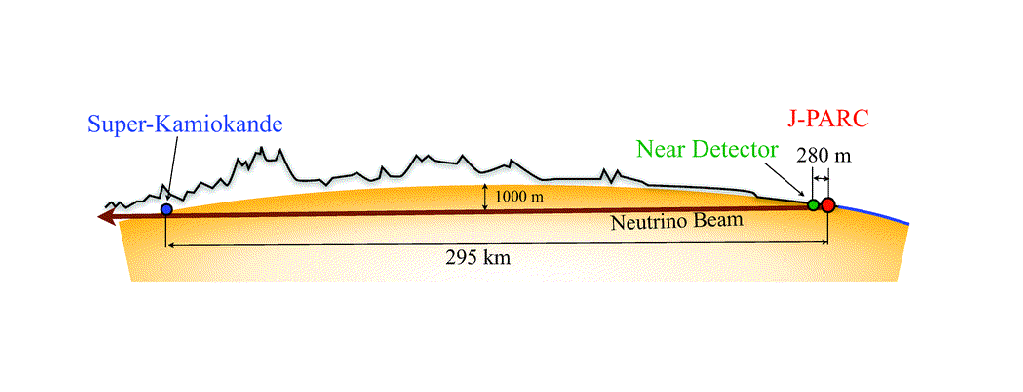
\includegraphics[width=0.98\textwidth]{images/t2k/journey_of_T2K_Neutrino-5.eps}
  \caption[Overview of the T2K experiment]{Overview of the
    \Gls{TK} experiment (not to scale). Taken from~\cite{T2K2011}.}
  \label{fig:t2k}
\end{figure}

The Tokai to Kamioka (\Gls{TK}) experiment~\cite{T2K2011}, represented
in Figure~\ref{fig:t2k}, was designed to measure
$\sin^2(2\theta_{13})$ via electron (anti-) neutrino (\gls{nue} and
\gls{anue}) appearance in a muon $\mbox{(anti-)}$ neutrino (\gls{numu}
and \gls{anumu}) beam~\cite{T2K2011}. Neutrino and anti-neutrino
measurements can lead to hints of a possible non-zero
$\sin(\Delta \delta_{\text{CP}})$ which would indicate violation of
Charge Parity (\Gls{CP}) in the lepton sector. This is one of the
remaining parameters of particle physics that has not been measured
yet. \Gls{TK} also measures $\sin^2(\theta_{23})$ via muon (anti-)
neutrino disappearance~\cite{Abe:2017vif}.

To do this, it uses an off-axis neutrino beam and a far detector,
Super-Kamiokande (\Gls{SK}), placed off-axis at $295$~km from the
Japan Proton Accelerator Research Complex (\Gls{JPARC}) and a beam
energy of $600$~MeV, such that the $\nu_\mu$ to $\nu_\mu$
disappearance probability is maximum; the peak energy also coincides
with the energy where the \Gls{CCQE} processes are the most likely to
happen.

Two other detectors (the Interactive Neutrino GRID, \Gls{INGRID} and
the off-axis Near Detector, \Gls{ND}) are located $280$~m away from
the target and are used for beam and cross section measurements.

In all this thesis, unless stated otherwise, the Z direction refers to
the direction between the target and the far detector (with the
positive direction being towards the far detector), the X direction is
the horizontal direction and Y is the vertical direction (positive Y
being upwards).

\section{T2K Beamline}
\label{sec:t2kbeamline}
The neutrino beam is created by impinging 30~GeV protons on a carbon
target at the \Gls{JPARC} facility in Tokai,
Japan~\cite{FluxT2K2013}. This produces pions and kaons that mainly
decay into muons and neutrinos, as can be seen in the listing in
Table~\ref{tab:nudecaymode}. In Figure~\ref{fig:oaeffect}, the beam
spectrum for different off-axis angles of the neutrino beam is shown.
This technique was developed in 1995 at BNL~\cite{AGS1993}.  The main
idea is to use the 2 body decay kinematics of the hadron to predict
the neutrino energy, which comes from considering the energy and
momentum conservations equation of a pion decaying to a neutrino and a
charged lepton:
\begin{equation}
  E_\nu = \frac{m_\pi^2 - m_\mu^2}{2(E_\pi - p_\pi\cos\theta_\nu)}.
  \label{eq:offaxis}
\end{equation}
Assuming that the parents of the neutrino are mainly pions of mass
$m_\pi$, energy $E_\pi$ and momentum $p_\pi$; they decay into a muon
of mass $m_\mu$ and a neutrino of energy $E_\nu$ and angle
$\theta_\nu$ with respect to the pion trajectory.

When one integrates the pion kinematics from the pion energy
distribution, it can be found that the energy distribution of the
neutrinos also becomes more peaked (smaller width of the distribution)
for increasing off-axis. This effect is visible in
Figure~\ref{fig:oaeffect}: increasing the off-axis angle of the
neutrinos reduces the peak energy of the neutrino flux and the width
of the neutrino energy distribution. At \Gls{TK}, the \gls{numu} beam
whose energy is centred at \energy when viewed from an off-axis angle
of \offaxis as seen on Figure~\ref{fig:oaeffect}. This angle was
optimised to maximise the disappearance probability of the muon
neutrino as can be seen in top of Figure~\ref{fig:oaeffect}.

\begin{figure}[ht]
  \begin{center}
    \includegraphics[keepaspectratio=true,width=0.58\textwidth]{images/t2k/oaeffect_flux.pdf}
    \caption[Muon neutrino survival probability assuming maximal
    mixing and $\Delta m^2_{32}=2.4\times 10^{-3}\text{~eV}^2$ at
    SK. Neutrino flux energy distribution for different off-axis at
    295~km]{\textbf{\textit{Top:}} Muon (anti-) neutrino survival
      probability at \Gls{SK} (295~km), against neutrino energy
      assuming maximal mixing ($\sin^22\theta_{23} = 1$) and
      $\Delta m^2_{32}=2.4\times
      10^{-3}\text{~eV}^2$. \textbf{\textit{Bottom:}} \Gls{TK}
      neutrino flux energy distributions for different off-axis
      angles. Taken from~\cite{FluxT2K2013}.}
    \label{fig:oaeffect}
  \end{center}
\end{figure}

\begin{table}[ht]
  \begin{center}
    \begin{tabular}{rlc}
      \toprule
      Particle & Decay products & Branching fraction ($\%$) \\
      \midrule
      $\pi^{+}$ & $\rightarrow \mu^{+}\nu_{\mu}$ & $99.9877$ \\
               & $\rightarrow e^{+}\nu_{e}$ &  $1.23\times10^{-4}$\\
      K$^{+}$ &  $\rightarrow \mu^{+}\nu_{\mu}$ & $63.55$ \\
               &  $\rightarrow \pi^{0}\mu^{+}\nu_{\mu}$ & $3.353$ \\
               &  $\rightarrow \pi^{0}e^{+}\nu_{e}$ & $5.07$ \\
      K$_L^{0}$ & $\rightarrow \pi^{-}\mu^{+}\nu_{\mu}$ & $27.04$ \\
               & $\rightarrow \pi^{-}e^{+}\nu_{e}$ & $40.55$ \\
      $\mu^{+}$ & $\rightarrow e^{+}\bar{\nu}_{\mu}\nu_{e}$ & $100$ \\
      \bottomrule
    \end{tabular}
    \caption[Neutrino-producing decay modes considered in T2K's flux
    simulation]{Neutrino-producing decay modes considered in
      \Gls{TK}'s flux simulation and their branching ratio in
      percentage.  Decay modes for \gls{anumu} and \gls{anue} are
      omitted in this table, but can be derived by taking the charge
      conjugate of the $\pi^{-}$, K$^{-}$ and $\mu^{-}$
      modes. Reproduced from~\cite{FluxT2K2013}.}
    \label{tab:nudecaymode}
  \end{center}
\end{table}

At \gls{JPARC}, the production of the neutrino beam is realised in 3
stages:
\begin{itemize}[noitemsep,topsep=0pt]
\item first, protons are accelerated in the \gls{JPARC} accelerator;
\item then, they are monitored and transported to the target in the
  primary beamline;
\item finally, once the protons hit the target, the hadrons produced
  are propagated in the secondary beamline.
\end{itemize}
The three parts leading to the creation of the neutrino beam are now
described.

\subsection{J-PARC accelerator}
\label{subsec:jparcaccelerator}
The \Gls{JPARC} accelerator consists of one linear accelerator
(\Gls{LINAC}) and two synchrotrons (\Gls{RCS} for Rapid Cycling
Synchrotron and \gls{MR} for Main Ring). The \Gls{LINAC} is 300~m long
and accelerates $H^-$ up to 181~MeV. These $H^-$ are converted to
protons by charge-stripping foils while entering the RCS. The protons
are then accelerated to 3~GeV, and then injected in the \Gls{MR} to be
accelerated to 30~GeV. At this point, 8 bunches are circulating in the
\Gls{MR}, and each of these contains roughly $3\times 10^{14}$
protons.  These 8 bunches are then ``kicked'' (i.e. deviated) by
magnets to go into the primary beamline. This process is repeated
every $2\sim 3$~seconds to create spills.  The time between two
bunches in the same spill is $\sim 600$~ns.  Short spills allow
efficient rejection of cosmogenic particles at the \Gls{ND} and
\Gls{SK}.

\subsection{Primary beamline}
\label{subsec:primarybeam}

\begin{figure}[ht]
  \center
  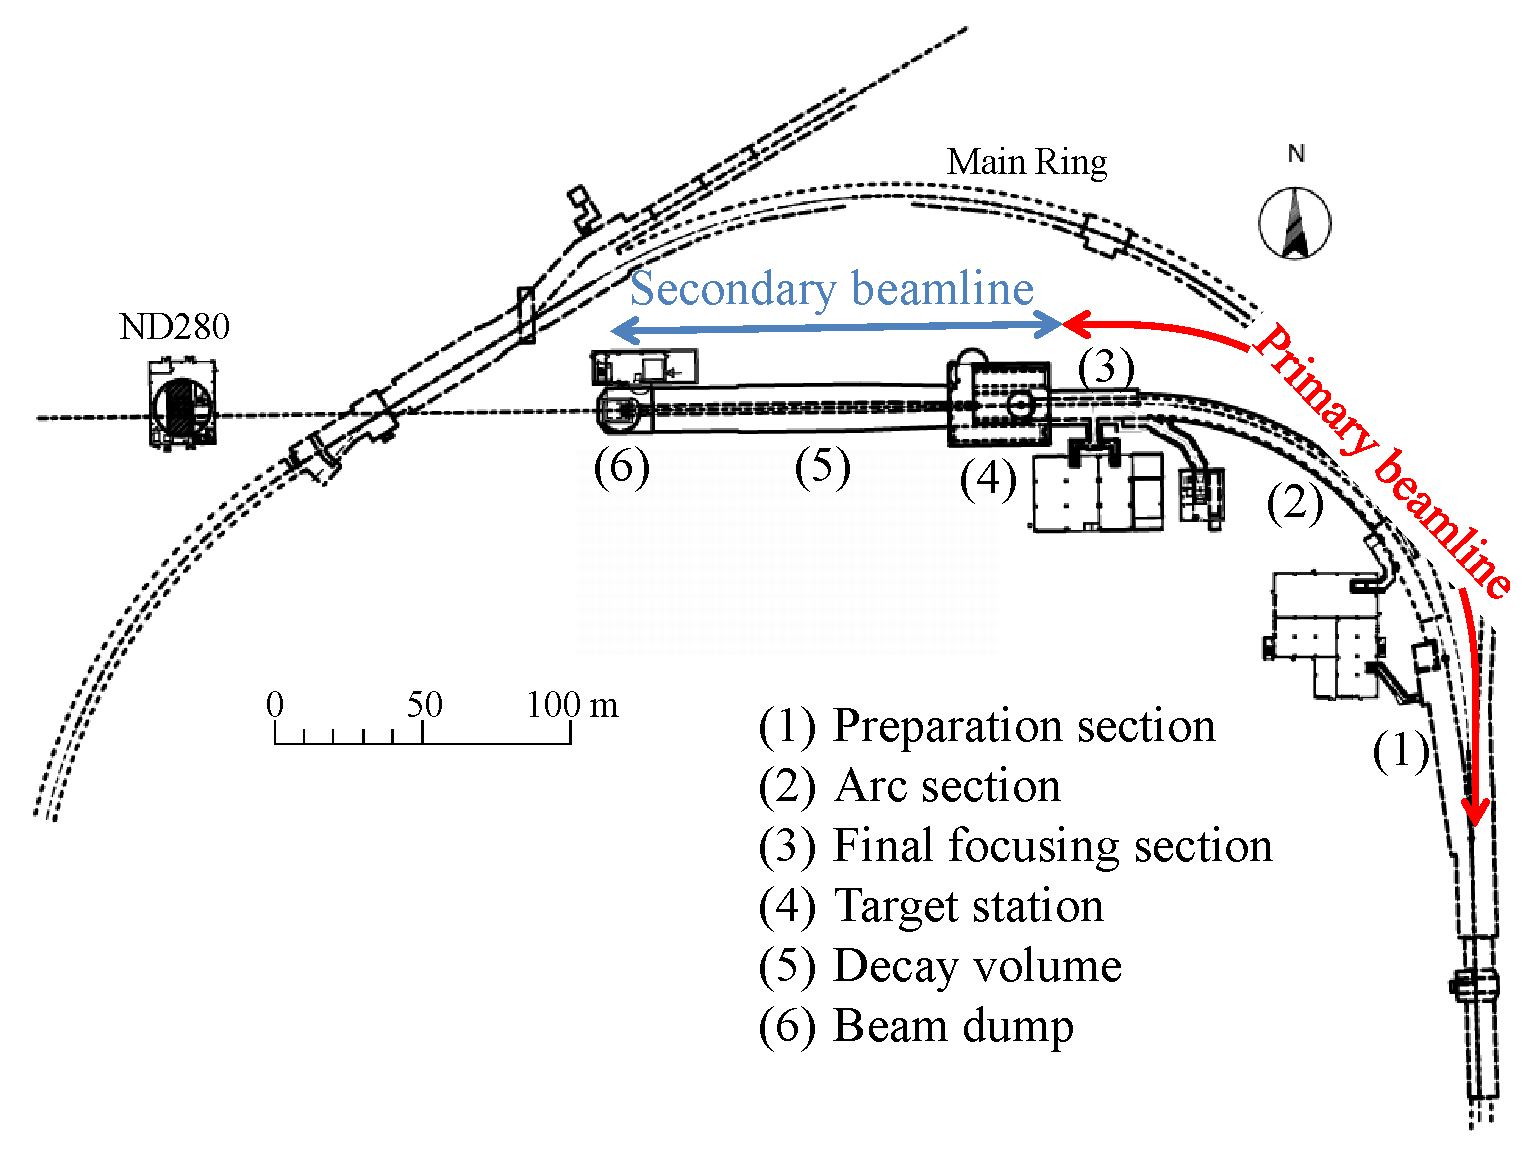
\includegraphics[width=0.6\textwidth]{images/t2k/beamline.eps} \\
  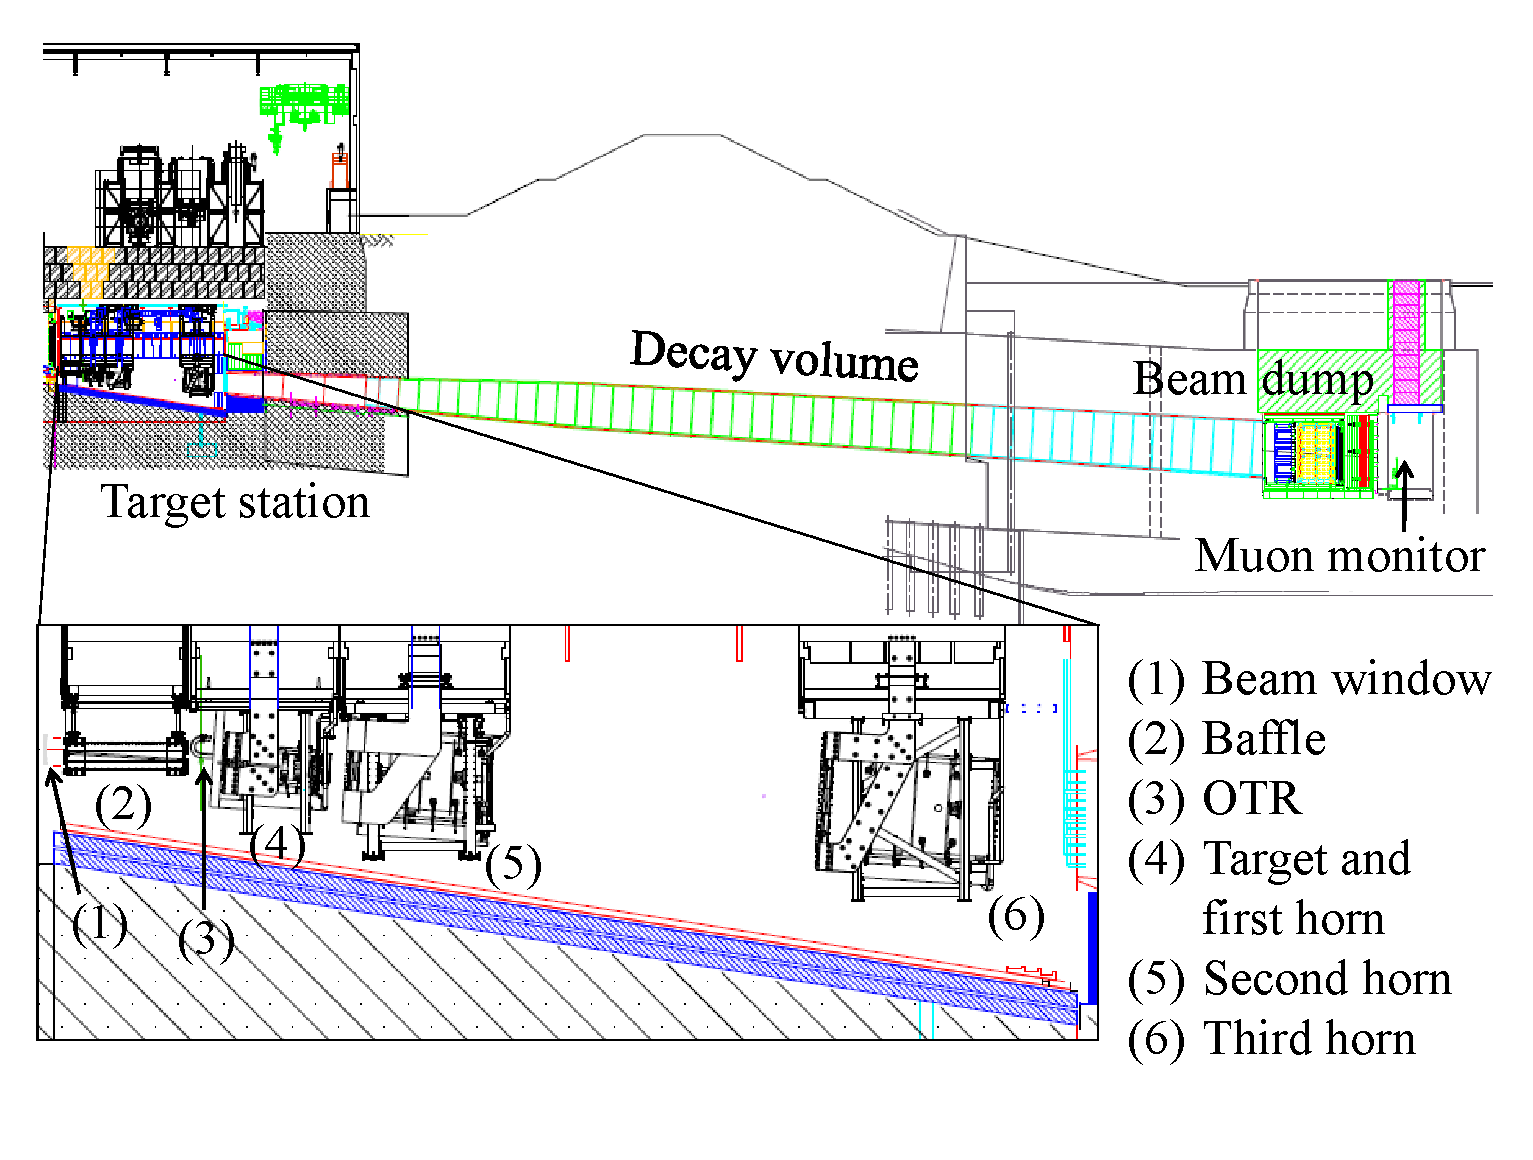
\includegraphics[width=0.6\textwidth]{images/t2k/beamline_sec.eps}
  \caption[Beamline and secondary beamline at
  J-PARC]{\textbf{\textit{Top:}} Beamline at
    \Gls{JPARC}. \textbf{\textit{Bottom:}} Secondary beamline. Taken
    from~\cite{FluxT2K2013}.}
  \label{fig:beamline}
\end{figure}

The whole beamline is represented on the left of
Figure~\ref{fig:beamline}. The primary beamline consists of a
preparation section of 54~m which contains eleven magnets (four
steering magnets, two dipole magnets, and five quadrupole magnets to
focus the beam), an arc-section of 147~m composed of fourteen
superconducting magnets to bend the beam by $\sim 80^{\circ}$, and a
final focusing section (37~m). This last section directs the beam
downwards and focuses the beam on the target; it contains ten magnets
(four steering magnets, two dipole magnets and four quadrupole
magnets).

The primary beamline is instrumented to monitor the proton intensity,
position, profile and losses.

The proton intensity stability measurement is done by five current
transformers (\Glspl{CT}) around the beam. Schematic representation of
a \Gls{CT} is given on the left of Figure~\ref{fig:ssem}.

\begin{figure}[ht]
  \center
  \includegraphics[width=0.6\textwidth]{images/t2k/ct.png} \\
  \includegraphics[width=0.6\textwidth]{images/t2k/ssem.png}
  \caption[Illustration of a CT and a SSEM]{\textbf{\textit{Top:}}
    Illustration of a \Gls{CT}. \textbf{\textit{Bottom:}} A
    \Gls{SSEM}. Taken from~\cite{Hartz}.}
  \label{fig:ssem}
\end{figure}

There are fourty Beam Loss Monitors (\Glspl{BLM}), which are gaseous
detectors around the beamline. They are able to detect protons
escaping from the beam which ionise the gas. The \Glspl{BLM} can
trigger an interlock which stops the operations of the beam if the
losses exceed a certain threshold value.

Nineteen \Glspl{SSEM} (Segmented Secondary Emission Profile Monitors)
are located in the beam pipe. They consist of strips oriented in the X
and Y directions placed in front of an anode foil; a bias voltage is
then applied between the strips and the anode. When the beam goes
through, it creates electrons on the strips that are accelerated to
the anode. This process generates a current on each strip directly
proportional to the number of protons crossing it. An illustration of
the device is given on the right of Figure~\ref{fig:ssem}. Because the
\Glspl{SSEM} are destructive of the proton beam and lead to
unacceptable beam loss, they are movable and are only used at specific
times, during the so-called ``beam tuning'' runs. In normal physics
runs, only the last \Gls{SSEM} is used.

Finally, twenty-one \Glspl{ESM} (Electro-Static Beam Position Monitor)
are located near the \Gls{SSEM} to measure the electrostatic shape of
the beam; these are capacitors which give access to the position of
the beam in the beam pipe.

\subsection{Secondary beamline}
\label{subsec:secondarybeam}
The most upstream components of the secondary beamline are in the
target station. It contains the \Gls{OTR} (Optical Transition
Radiation Monitor), which is a device composed of a foil that produces
radiation and fluorescent light when the beam crosses it.  This is
imaged using mirrors and a camera. This device has access to the beam
position and size before it hits the target, 280~mm downstream of it.

The target is a graphite cylinder. Its length is 91.4~cm and its
diameter 2.6~cm. The size and material have been carefully designed to
resist the heat wave generated by the high intensity proton bunches
impinging it. The target is surrounded by an inert helium vessel (15~m
in length, 4~m in width and 11~m in height).

The other parts of secondary beamline are downstream of the carbon
target, i.e. they manipulate and monitor the hadrons produced by the
proton collision on the target. This part is represented on the right
hand side of Figure~\ref{fig:beamline}.

Downstream of the target station, one finds a decay volume for the
hadrons. It is an empty 96~m long steel tunnel, which measures 1.4~m
wide upstream and 3.0~m wide downstream, whereas the height is
increased from 1.7~m to 5.0~m between the upstream and the downstream
part.

Finally, the beam dump is downstream of the decay tunnel. It is used
to stop the muons and the hadrons that have not decayed in the
tunnel. The MUon MONitor (MUMON) is placed just after the beam dump to
detect the muons going through.

Three magnetic horns are placed around the secondary beamline. The
first one is around the target station and serves to collect the
pions. The second and third ones focus the pions. In neutrino mode,
these horns operate at 250~kA and produce a magnetic field of up to
1.7~T (so-called Forward Horn Current, \Gls{FHC}). The current can be
reversed to focus negative pions and produce an anti-neutrino beam
(Reverse Horn Current, \Gls{RHC}). The effect of the horns is to
increase 17-fold the neutrino flux at the far detector. They also
provide better rejection of wrong sign hadrons which produce
background neutrinos for oscillation analysis, making them fundamental
parts of the \Gls{TK} experiment. The beam composition at the off-axis
near detector is shown in Table~\ref{tab:flavor_frac}.

\begin{table}[ht]
  \center
  \tabcolsep=0.11cm
  \begin{tabular}{lccccc}
    \toprule
    \multicolumn{2}{c}{Energy Range [GeV]} & $0$ to $1.5$ & $1.5$ to $3.0$ &  greater than $3.0$ & all \\ 
    \midrule
    Beam mode & Flavour & \multicolumn{4}{c}{Proportion: relative (total)} \\
    \midrule
    \multirow{4}{*}{Neutrino}
                                           & \gls{numu}  & $93.8\%   (84.9\%)$   & $81.7\%  (4.55\%)$   & $88.6\% (3.49\%)$  & $92.9\% $  \\
                                           & \gls{anumu} & $5.23\%   (4.74\%)$   & $14.1\%  (0.784\%)$  & $7.97\% (0.314\%)$ & $5.83\% $  \\
                                           & \gls{nue}   & $0.869\%  (0.786\%)$  & $3.44\%  (0.192\%)$  & $2.8\%  (0.11\%)$  & $1.09\% $  \\
                                           & \gls{anue}  & $0.0852\% (0.0771\%)$ & $0.787\% (0.0439\%)$ & $0.66\% (0.026\%)$ & $0.147\% $ \\
    \midrule
    \multirow{4}{*}{Anti-neutrino}
                                           & \gls{numu}  & $7.07\%  (6.53\%)$  & $32.7\% (1.68\%)$   & $42.4\% (1.09\%)$   & $9.3\% $   \\
                                           & \gls{anumu} & $92\%    (84.9\%)$  & $63.8\% (3.29\%)$   & $53.5\% (1.37\%)$   & $89.5\% $  \\
                                           & \gls{nue}   & $0.131\% (0.121\%)$ & $1.37\% (0.0705\%)$ & $2.07\% (0.0529\%)$ & $0.244\% $ \\
                                           & \gls{anue}  & $0.83\%  (0.766\%)$ & $2.17\% (0.112\%)$  & $1.97\% (0.0505\%)$ & $0.929\% $ \\
    \bottomrule
  \end{tabular}
  \caption[Fraction of the total flux by flavour]{Fraction of the
    total flux by flavour in bins of the neutrino energy when running
    in neutrino mode (run 4) and anti-neutrino mode (run 5) at the
    off-axis near detector (\Gls{ND}). The fractions in parentheses
    are relative to the total flux over all neutrino
    energies. Extracted from the neutrino flux prediction from the
    \Gls{TK} beam group~\cite{TomislavVladisavljevicFluxTuning2017}.}
  \label{tab:flavor_frac}
\end{table}

After simulation and including the constraints from the replica target
measurements at the NA61~/~SHINE
experiments~\cite{Abgrall:2011ae,Abgrall:2011ts,Abgrall:2015hmv}, the
flux uncertainty reaches $\sim8\%$ at the energy peak and the
different components of the flux can be estimated as a function of the
neutrino energy for neutrino and anti-neutrino modes, as can be seen
in Figures~\ref{fig:flux1} and \ref{fig:flux2}. This uncertainty is
expected to decrease as more data from NA61~/~SHINE are analysed.

\begin{figure}[ht!]
  \center
  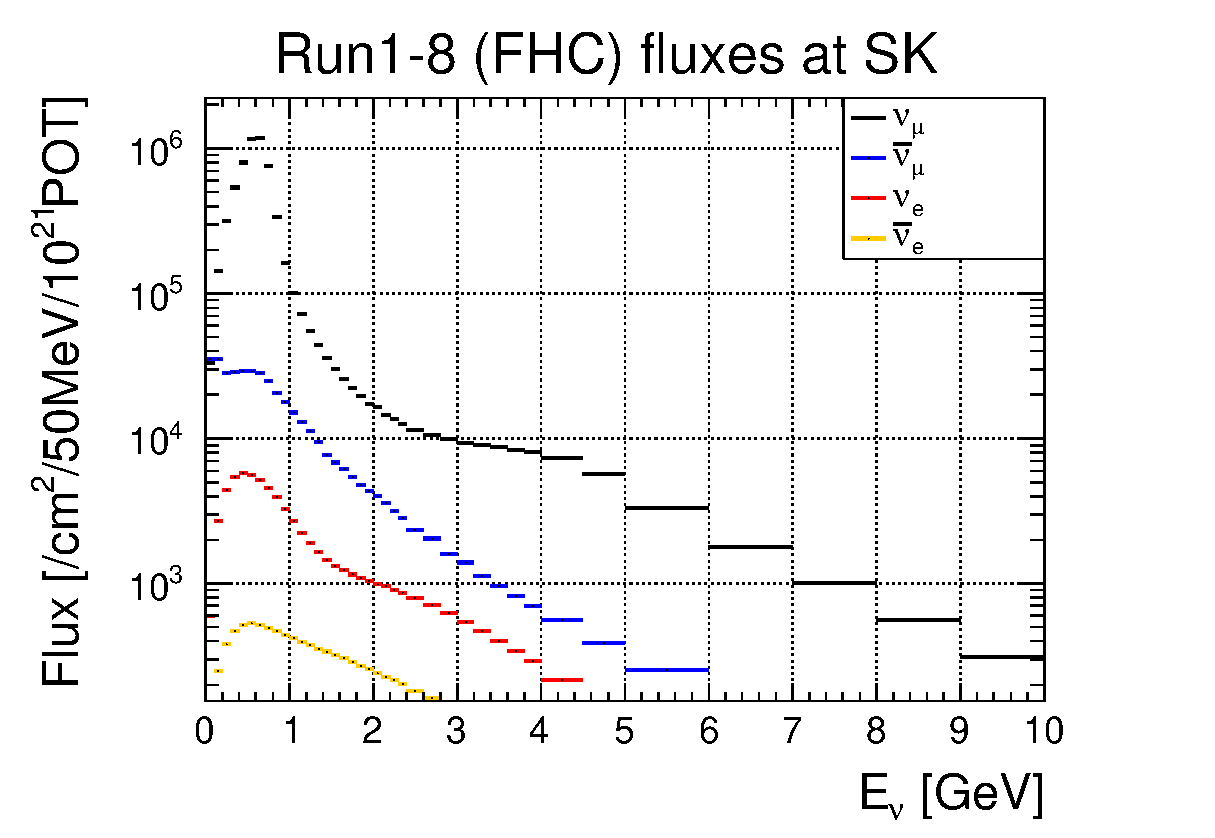
\includegraphics[width=0.6\textwidth]{images/t2k/SK_FHC_flux.eps} \\
  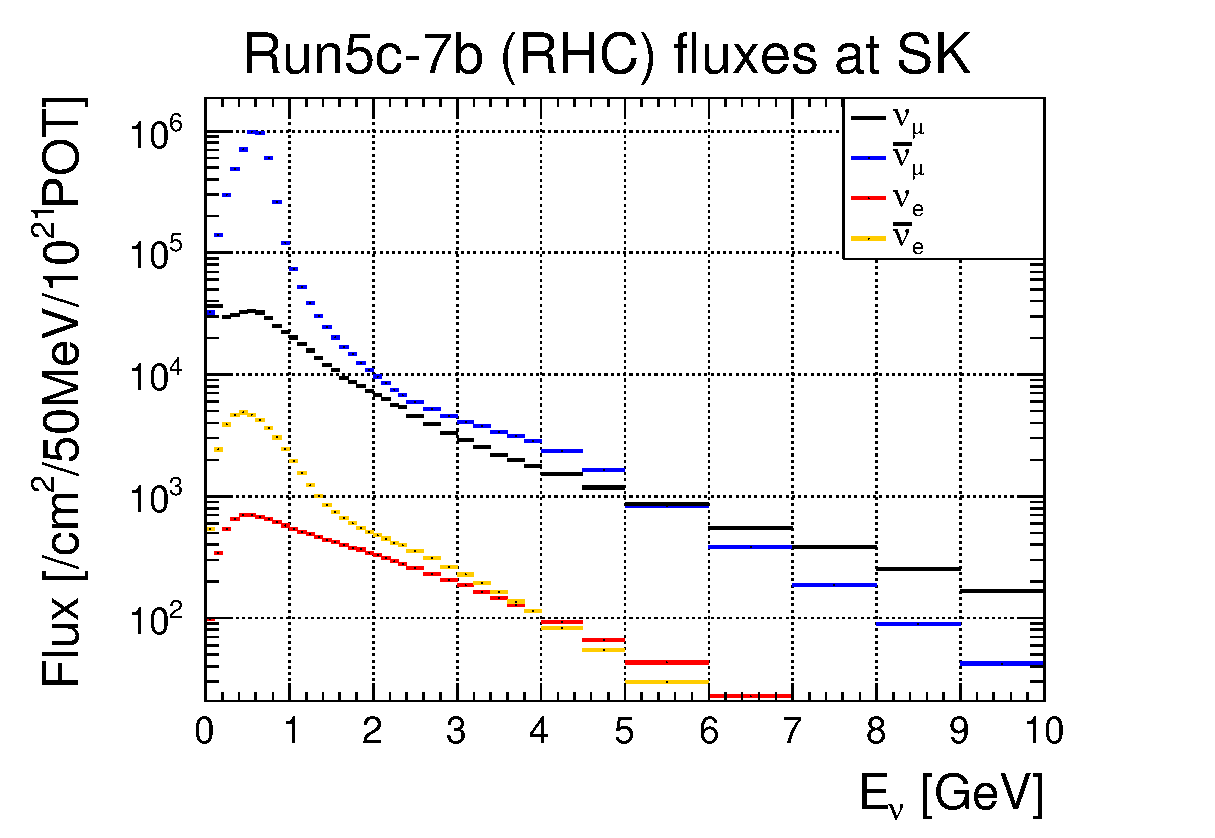
\includegraphics[width=0.6\textwidth]{images/t2k/SK_RHC_flux.eps}
  \caption[Neutrino flux prediction in (anti-) neutrino
  mode]{\textbf{\textit{Top:}} Neutrino flux prediction in neutrino
    mode. \textbf{\textit{Bottom:}} Neutrino flux in anti-neutrino
    mode. Extracted from the neutrino flux prediction and errors from
    the \Gls{TK} beam
    group~\cite{TomislavVladisavljevicFluxTuning2017,MarkHartzFluxUncertainty2017}.}
  \label{fig:flux1}
\end{figure}

\begin{figure}[ht!]
  \center
  \includegraphics[width=0.6\textwidth]{images/t2k/SK_numode.eps} \\
  \includegraphics[width=0.6\textwidth]{images/t2k/SK_anumode.eps}
  \caption[Neutrino flux prediction errors in (anti-) neutrino
  mode]{\textbf{\textit{Top:}} Diagonal uncertainties on the
    \gls{numu} flux in neutrino mode at \Gls{SK}, overlaid with the
    neutrino rate (cross section times flux) \textbf{\textit{Bottom:}}
    Diagonal uncertainties on the \gls{anumu} flux in anti-neutrino
    mode at \Gls{SK}, overlaid with the neutrino rate. Extracted from
    the neutrino flux prediction and errors from the \Gls{TK} beam
    group~\cite{TomislavVladisavljevicFluxTuning2017,MarkHartzFluxUncertainty2017}.}
  \label{fig:flux2}
\end{figure}
\clearpage

\section{Near detectors}
\label{sec:neardetectors}
The near detector suite is composed of 2 detectors, \Gls{INGRID} and
\Gls{ND}. Both of them are in the so-called ``pit''
(Figure~\ref{fig:pit}). Their designs are described here.

\begin{figure}[ht]
  \center
  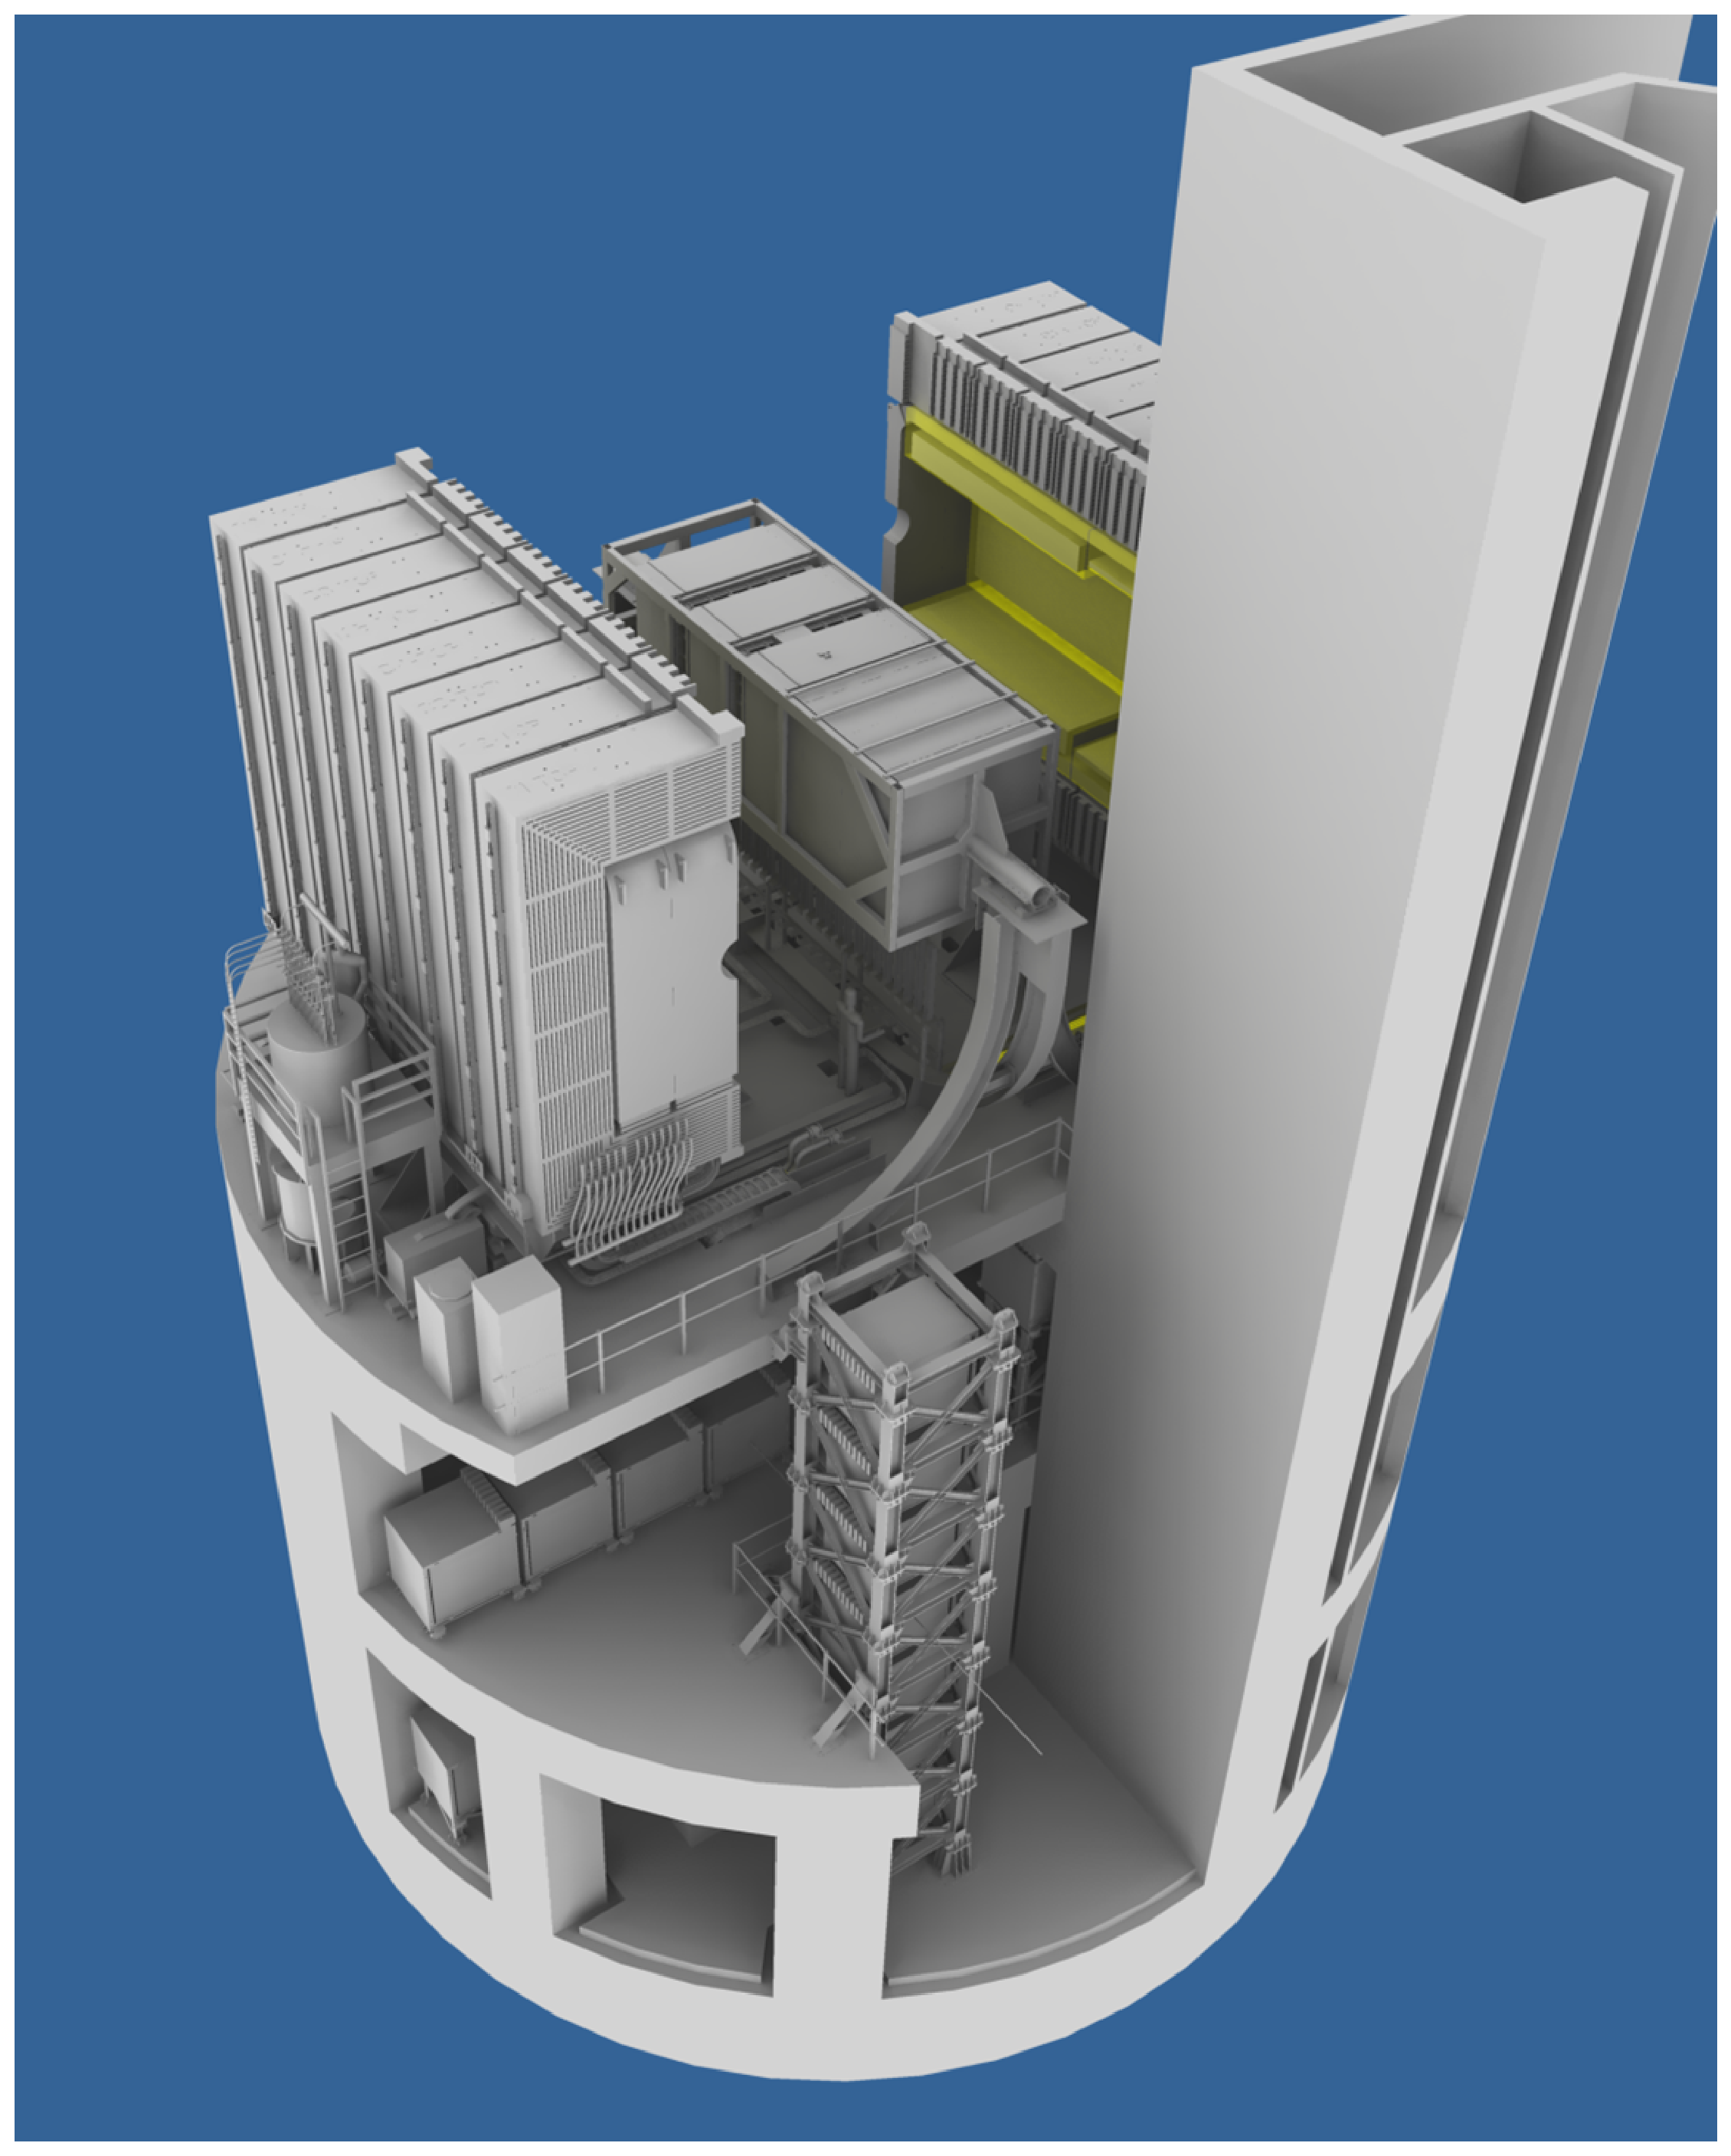
\includegraphics[width=0.48\textwidth]{images/t2k/ND280Pit.eps}
  \caption[Near detector complex]{Near detector complex of the
    \Gls{TK} experiment. On the top, the off-axis near detector at 280
    metres (\Gls{ND}) can be seen in open configuration; in the
    bottom, the Interactive Neutrino GRID (\Gls{INGRID}) cross
    structure can be seen. Taken from~\cite{T2K2011}.}
  \label{fig:pit}
\end{figure}

\subsection{Interactive Neutrino GRID}
\label{subsec:ingrid}
The \Gls{INGRID} (Interactive Neutrino GRID) detector is composed of
sixteen modules. They are placed in a cross structure as shown in
Figure~\ref{fig:INGRID}. The centre of the cross corresponds to the
centre of the beam. \Gls{INGRID}'s primary purpose is to monitor the
beam centre. A 10~cm precision is required to get a 0.4~mRad precision
in the direction of the beam which is an important input to know the
peak energy as shown earlier in Equation~\ref{eq:offaxis}.

\begin{figure}[ht]
  \center
  \includegraphics[width=0.48\textwidth]{images/t2k/ingrid.pdf}
  \caption[INGRID detector]{\Gls{INGRID} detector of the \Gls{TK}
    experiment. Taken from~\cite{T2K2011}.}
  \label{fig:INGRID}
\end{figure}

All the modules have the same design. They consist of nine iron layers
of $124 \times 124 \times 6.5\text{~cm}^{3}$ providing a total target
mass of 7.1~t for each module. These iron layers are alternated with
eleven scintillator layers.  Each one of these layers is made with
forty-eight bars oriented both in X and Y directions (perpendicular to
the beam axis). This cube is surrounded by a veto region made of
twenty-two scintillator bars oriented in the Z direction. All the
scintillators have a wavelength shifting fibre (\Gls{WSF}) going
through the centre to collect the light produced by the particles. The
scintillators are made of polystyrene doped with \Gls{PPO} and
\Gls{POPOP} (which emits UV light from charged particle and shifts the
light frequency to enhance the light absorption on the fibre,
respectively). They have a rectangular cross section of
$1.0 \times 5.0\text{~cm}$ and are co-extruded with reflective
material ($TiO_2$) to reflect escaping photons, thus reducing
cross-talk between bars and enhancing the photon collection yield on
the fibre.

In addition, a ``proton module'' was designed to study the protons
from \gls{numu} interactions. The difference with the other module is
that it has finer scintillator bars and no iron layer, which improves
the tracking capabilities for short proton tracks. It is located
between the two central modules.

The readouts were provided by the Hamamatsu company. They are
Multi-Pixel Photon Counters (\Glspl{MPPC}). These photosensors are
connected to the \Gls{WSF} which collects the light inside the
scintillators. This set-up provides the timing and the detected light
which are used to reconstruct the particles' trajectories, charge and
momentum.

\subsection{Multi-Pixel Photon Counter}
\label{subsec:mppc}
The Mutli-Pixel Photon Counters (\Glspl{MPPC}\footnote{\Gls{MPPC} is a
  trademark of Hamamatsu Photonics, the \Glspl{MPPC} used at the
  \Gls{TK} are the model S10362-13-050C~\cite{MPPC}.}, also referred
as Silicon photo-multiplier, \Gls{SiPM}) are elementary parts of the
near detectors at \Gls{TK}. They are used in all the scintillator
detectors and are the readout for the photons from the
\Gls{WSF}\footnote{of reference: Kuraray Y11 (200) S-35
  J-type~\cite{T2K2011}.}. A single \Gls{MPPC} measures
$1.3\times 1.3 \text{~mm}^2$ and contains 667 individual pixels. The
\Gls{MPPC} pixels are avalanche photodiodes.

In the Geiger regime, which is the one the \Gls{MPPC} are opperated
at, the output charge of the diode does not depend on the number of
the photoelectrons that have fired the pixel, and the output charge is
given by the simple relation:
\begin{equation}
  Q=C(V-V_{\text{BD}}),
\end{equation}
where $Q$ is the output charge, $C$ ($\simeq60\text{pF}$) is the
internal capacity of the diode and $V$ is the applied bias voltage and
$V_\text{BD}$, the breakdown voltage, which is around $70\text{V}$.
This set-up gives a gain of about $10^5\sim 10^6$ (nominally
$7.5\times 10^5$). Note that the breakdown voltage is dependent on the
ambient temperature (typically $50\text{~mV}/^\circ\text{C}$), so a
change of few degrees can significantly modify the gains. The value of
the gain has to be calibrated for each period of roughly constant
temperature.

Since the pixels have a binary response (0 or 1 depending if the pixel
was hit), this allows to count photo-electrons depending on the number
of fired pixels. The charge deposited in the scintillator bar is
roughly proportional to the number of pixels hit.

\subsection{Off-Axis Near Detector at 280 meters}
\label{subsec:nd280}
\begin{figure}[ht]
  \center
  \begin{overpic}[width=0.6\linewidth]                {./images/t2k/ND280Exploded-Text-White.eps}
    \put(55,55){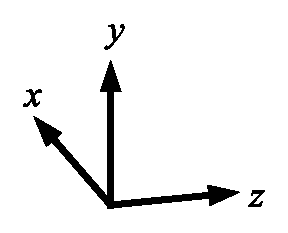
\includegraphics[width=0.12\linewidth]{./images/t2k/ND280-Coord-xyz.eps}}
    \put(0,20) {\includegraphics[width=0.1\linewidth ]{./images/t2k/ND280-Coord-Beam.eps}}
  \end{overpic}

  % 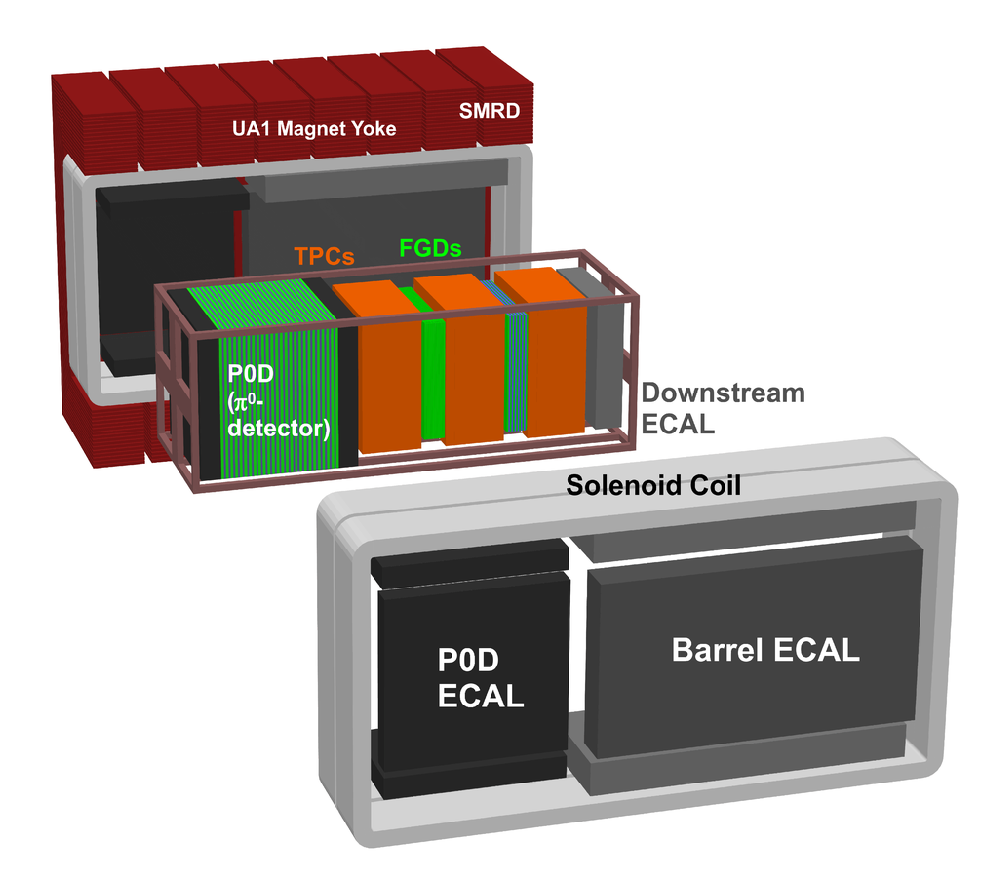
\includegraphics[width=0.68\textwidth]{images/t2k/ND280Exploded-Text-White.eps}
  \caption[Exploded view of the ND280]{Exploded view of the \Gls{ND}
    of the \Gls{TK} experiment, with its coordinate system and beam
    direction. Taken from~\cite{T2K2011}.}
  \label{fig:nd280}
\end{figure}

The off-axis Near Detector at 280 metres (\Gls{ND}), which is used in
the analyses described in this thesis, is a composite detector
enclosed in a magnet. The \Gls{ND} is illustrated on
Figure~\ref{fig:nd280}. It is placed at a $2.5^{\circ}$ off-axis angle
to have the closest neutrino energy distribution to the one in the far
detector. The description of the detector is made from the most
outward to inward regions and upstream to downstream, where upstream
refers to closest position to the target (left of
Figure~\ref{fig:nd280}).

\subsubsection{UA1 Magnet}
\label{subsubsec:magnet}
The magnet consists of aluminium coils circulating around the \Gls{ND}
as can be seen in light grey on Figure~\ref{fig:nd280}. They create a
horizontal dipole field of $0.2$~T. The return yoke (in red) and coils
were reused from the UA1 and the \Gls{NOMAD} experiments at CERN. The
yoke is composed of 2 C-shaped half yokes, that provide magnetic
insulation for the surrounding of the detector. The yoke is used as a
muon spectrometer and contain the magnetic field inside the inner
region of the detector due to their low saturation field. Both halves
are placed on rails that open to allow reach of the inner region. This
is visible in Figure~\ref{fig:pit}.

The magnetic field is a central part in the particle identification
with the Time Projection Chambers as will be shown later, so the field
was carefully calibrated in the whole detector before the inner parts
of the detector were placed inside it.

\subsubsection{Side Muon Range Detector}
\label{subsubsec:smrd}
The Side Muon Range Detector (\Gls{SMRD})~\cite{SMRD} is placed inside
the yoke and can identify escaping muons from neutrino interactions
inside the inner detector. It also serves as veto (or trigger) for
cosmic muons.  It is composed of 2008 scintillator bars with coarse
granularity ($7 \times 175 \times 875 \text{mm}^{3}$) oriented
horizontally and vertically.

\subsubsection{Pi~Zero Detector}
\label{subsubsec:p0d}
The Pi~Zero detector (\Gls{PD})~\cite{POD} is a scintillator detector
that was designed to measure the neutrino cross section of neutral
pion (\gls{piz}) production on water. As scintillator offers better
resolution than water, the idea is to have bags that can be filled
with water between the scintillator bars. One can make two
measurements: one with water in the bag and another one without
water. Both measurements can be used simultaneously to get a cross
section on water only.

The \Gls{PD} is made of fourty modules each containing 134 vertical
and 126 horizontal scintillator bars, alternating with brass as
depicted on Figure~\ref{fig:pod}. This set-up is realised to damp the
\Gls{EM} showers. The scintillator bars have very similar design to
the ones in the \Gls{INGRID} detector (\Gls{PPO} and \Gls{POPOP}
doped, coated with $TiO_2$, using a \Gls{WSF} and \Gls{MPPC} readout),
except their triangular cross section as can be seen in the insert of
Figure~\ref{fig:pod}. Their sizes are 33~mm at the base of the
triangle, 17~mm for the height, similarly to what was done for the
\Gls{MINERVA} neutrino experiment.

In the upstream and downstream parts of the \Gls{PD}, the water is
replaced by iron to contain the Electro-Magnetic (\Gls{EM}) showers.

\begin{figure}[ht]
  \center
  \includegraphics[width=0.6\linewidth]{images/t2k/p0d-schematic.eps}
  \caption[P0D of the ND280]{\Gls{PD} of the \Gls{ND} at the \Gls{TK}
    experiment. The neutrino beam is directed from the left to the
    right. Taken from~\cite{POD}.}
  \label{fig:pod}
\end{figure}

\subsubsection{Time Projection Chambers}
\label{subsubsec:tpc}
Going downstream from the \Gls{PD}, one finds the first Time
Projection Chambers (\Glspl{TPC})~\cite{TPC}. There are three
\Glspl{TPC} in what is loosely called the tracker region (composed of
the Fine Grained Detectors (\Glspl{FGD}) and \Glspl{TPC} region) of
the \Gls{ND}.

In the central part of the \Gls{TPC}, a cathode is polarised with a
strong negative voltage (-25~kV) which provides a drift field of
275~V/cm across the inner box.

The \Glspl{TPC} are filled with a mix of argon, $CF_4$ and
$i C_4H_{10}$ gas (where the $i$ stands for the ``iso'' isomer, which
means the molecule has a pyramidal configuration) at atmospheric
pressure.  This choice of pressure is to reduce the strains and
deflections on the side panels of the \Glspl{TPC}, as this would
distort the drift electric field in the chamber.  When a charged
particle enters the detector, it ionises the gas and the electrons,
typically a hundred electrons per cm are created in the gaseous argon
at atmospheric pressure. These ionisation electrons are drifted to a
charge detector (MicroMegas).  The drift time depends on the density
of the gas and is typically between $10-100~\mu\text{s}$.

The MicroMegas on the walls opposite to the cathode, record the
delayed pattern of the ionisation. A schematic view of a \Gls{TPC} is
shown in Figure~\ref{fig:tpc}. On each wall of the \Gls{TPC},
MicroMegas are aligned in 2 columns of 6 MicroMegas with a vertical
offset to avoid dead zones.  Each MicroMegas is composed of a Micro
Mesh Gaseous detector that amplifies the charge of the drifted
electron by applying a strong electric field ($\sim40\text{~kV/cm}$)
causing an electron avalanche (similar to an avalanche diode). The
MicroMegas amplifies the signal by a factor of about 2000. This gain
is inversely proportional to the pressure of the gas and thus the
current atmospheric pressure. The electrons from the cascade are then
read in the MicroMegas Pads, which is later called a hit. The size of
a MicroMegas is $342 \times 359 \text{~mm}^2$ and each of them is
meshed in a $36 \times 48$ array of pads, that have sizes of
$6.85 \times 9.65\text{~mm}^2$. This is the typical spatial resolution
for a charged particle crossing the detector.

The argon chamber is surrounded by another gas chamber filled with
carbon dioxide ($CO_2$) to insulate it electrically.

\begin{figure}[ht]
  \center
  %\includegraphics[width=0.6\textwidth]{images/t2k/tpc-eps-converted-to.pdf}
  \caption[Schematic view of the TPC in the ND280]{Schematic view of
    the \Gls{TPC} in the \Gls{ND}. Taken from~\cite{TPC}.}
  \label{fig:tpc}
\end{figure}

The \Gls{TPC} is a very precise detector that can be used for pointing
the particles and measuring their momentum in the magnetic field and
Particle IDentification (\Gls{PID}) by measuring the energy loss along
the trajectory ($dE/dx$) of the particle from the local curvature of
the trajectory in the magnetic field. This is visible in
Figure~\ref{fig:tpcdedx}, which shows the $dE/dx$ of the several
particles (positrons, anti-muons, positively charged pion and proton)
as measured in the \Gls{TPC} against their momentum.

\begin{figure}[ht]
  \center
  \includegraphics[width=0.6\textwidth]{images/t2k/dedx.pdf}
  \caption[TPC $dE/dx$ distributions for positively charged
  particles]{\Gls{TPC} $dE/dx$ for different ionising particles of
    positive charge in the \Gls{TPC}. Taken from~\cite{TPC}.}
  \label{fig:tpcdedx}
\end{figure}

\subsubsection{Fine Grained Detectors}
\label{subsubsec:fgd}
There are two Fine Grained Detectors (\Glspl{FGD})~\cite{FGD} in the
\Gls{ND}; they are placed in between the \Glspl{TPC}. Each \Gls{FGD}
is composed of scintillator bars which have small cross sections
($9.61 \times 9.61 \times 1864.3 \text{~mm}^3$). They are oriented in
the X and Y directions, alternately. Each scintillator bar has a
\Gls{WSF} in it and a \Gls{MPPC} associated at one end. It has the
same characteristics as those of the \Gls{INGRID} or \Gls{PD}.

When a Minimum Ionising Particle (\Gls{MIP}) enters one bar of the
\Gls{FGD}, it produces generally between ten to thirty photons. Most
of these enter the \Gls{WSF} and reach the \Gls{MPPC}. The
\Glspl{MPPC} amplifies the signal with a gain of about
$5\times 10^{5}$ to create a detectable charge.

Each of the thirty layers is composed of 192 bars, providing active
carbon target of 1.1~t. For the second \Gls{FGD}, six layers were
removed and filled with water to allow neutrino water cross section
measurement similar to what was described in \Gls{PD} section.

\subsubsection{Electromagnetic Calorimeter}
\label{subsubsec:ecal}
The whole \Gls{ND} tracker region (composed of the three Time
Projection Chambers and two Fine Grained Detectors) is surrounded by
an Electromagnetic Calorimeter (\Gls{ECal})~\cite{ECal}. This detector
was designed to measure \gls{piz} coming from neutrino interaction
inside the tracker region.

The \Gls{ECal} is composed of six modules surrounding the tracker
(\Gls{BrECal}, for barrel \Gls{ECal}) parallel to the Z direction, six
modules surrounding the \Gls{PD} (\Gls{P0DECal}) and another placed
after the third \Gls{TPC} (Downstream \Gls{ECal}, \Gls{DsECal}).  All
the \Gls{ECal} modules are made of scintillator bars. These bars have
a cross section of $4.0 \times 1.0 \text{~cm}^2$ and have with similar
specifications as the \Gls{PD}, \Gls{FGD} and \Gls{INGRID} bars. The
scintillator bars are alternated with lead layers to develop the
showers.

The \Gls{DsECal} is composed of thirty-four layers of lead alternated
with fifty layers of scintillator bars oriented in X and Y
directions. A similar design was made for the \Gls{BrECal}, with
thirty-one layers of lead.

The \Gls{P0DECal} is different because of the \Gls{PD} size and the
available space in the UA1 magnet. It only has five layers of lead and
six active layers of scintillator, all of which are oriented in the
same direction.

The \Gls{BrECal} and \Gls{DsECal} have an interaction length allowing
containment of all the showers
($\sim 10\text{X}_0$\footnote{$\text{X}_0$ is defined as the length
  for which an electron~/~photon has $sim 63\%$ chance to
  interact. This length is normalised by the density of the material
  its units are $\text{g} / \text{cm}^2$.}) whereas the \Gls{P0DECal}
cannot contain some of the showers due to its reduced size
($3.6 \text{X}_0$). The \Gls{P0DECal} was designed to veto external
particles.

Note that the \Gls{BrECal} and the \Gls{P0DECal} were placed in the
detector at the start of the run 2 of \Gls{TK}, over the summer 2011.


\section{The far detector: Super-Kamiokande}
\label{sec:sk}
The far detector (SuperKamiokande, \Gls{SK}) is located at 285~km away
from the graphite target at \Gls{JPARC}, in the Kamioka mine, on the
western cost of Japan~\cite{SK2003}. The mine is 1,000~m deep, under
the mount Ikenoyama, which is equivalent to roughly
2,700~m.w.e. (metre equivalent water).

The geometry of the detector is cylindrical (vertically), and the
vessel is made of stainless steel. A diagram of the detector is shown
in Figure~\ref{fig:sk}.  \Gls{SK} is composed of two coaxial cylinders
that define the inner volume and the outer volume. The inner detector
has a diameter of 33.8~m and the outer detector is 2~m wide. Its
height is 36.2~m. This provides a fiducial volume of 22.5~kton of
ultra-pure water.

\begin{figure}[ht]
  \center
  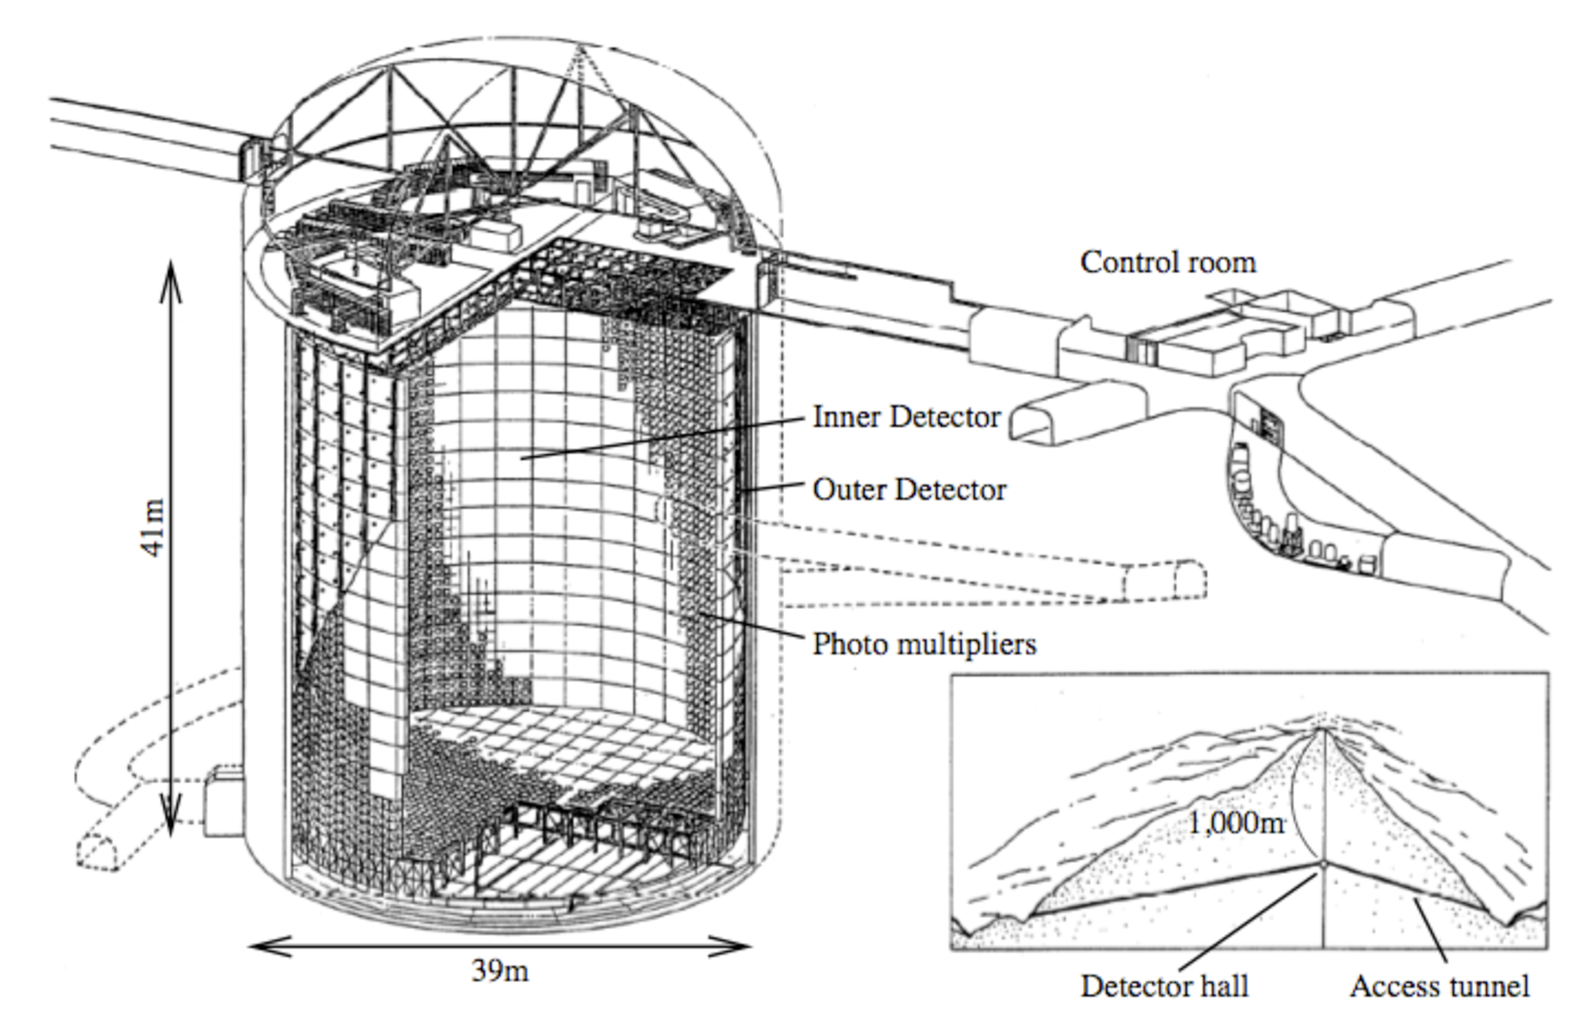
\includegraphics[width=0.8\textwidth]{images/T2K/SK_JHFDiagram.eps}
  \caption[SK detector]{Schematic view of the \Gls{SK} detector. Taken
    from~\cite{SK2003}.}
  \label{fig:sk}
\end{figure}

The inner detector is surrounded by 11,129 \Glspl{PMT} pointing
inwards of the detector, providing a 40\% photocoverage. The
\Glspl{PMT} detect the Cherenkov lights from charged particle after
neutrino interactions. There are also 1,885 \Glspl{PMT} pointing
outwards in the outer detector volume to veto events that happen
outside the detector. Each \Gls{PMT} can detect single photons. They
are sensitive to photons of wavelengths in the $350 - 500\text{~nm}$
range and the maximum quantum efficiency is reached for photons of
wavelength $\sim 400\text{~nm}$ (21~\% efficiency). The number of
photo-electrons is multiplied by a system of eleven dynodes of
Venetian blind type which are providing a gain of about $10^7$ when
operated at around $2~\text{kV}$, as is the case in
\Gls{SK}~\cite{SKPMT}.

Note that to produce Cherenkov light, a charged particle must
propagate at a velocity faster than the speed of light in the medium
it traverses. This means there is a threshold of energy for a particle
to be detected, which is given by $p>m/\sqrt{n^2-1}=m/1.27$, where $p$
and $m$ are the momentum and mass of the charged particle, and $n$ is
the refractive index of the medium, (1.3 in water).

In Figure~\ref{fig:cherenkov}, the signal produced by electrons and
muons from \Gls{TK} is shown. The somewhat simple design of the
detector allows a very efficient separation between muons and
electrons. Indeed, muons have a large mass ($105.6~\text{MeV}$) and
therefore propagate relatively straight in water. This is the reason
muons produce a clear Cherenkov ring on the \Gls{SK} wall. Electrons
on the other hand, because of their small mass, change direction and
produce \Gls{EM} showers when propagating (bremsstrahlung photons,
Compton scattering, pair production). They will produce a more poorly
defined (or ``fuzzier'') Cherenkov ring on the wall.

\begin{figure}[ht]
  \center
 % \includegraphics[width=0.8\textwidth]{images/T2K/numu_sk-eps-converted-to.pdf}\\
%  \includegraphics[width=0.8\textwidth]{images/T2K/nue_sk-eps-converted-to.pdf}
  \caption[Events observed at SK]{Events observed at
    \Gls{SK}. \textbf{\textit{Top:}} \gls{numu}
    candidate. \textbf{\textit{Bottom:}} \gls{nue} candidate. The
    Cherenkov light ring is ``fuzzier'' in the case of \gls{nue} due
    to multiple scatter of the electron. Both taken
    from~\cite{T2K2011}.}
  \label{fig:cherenkov}
\end{figure}

The detector can also detect delayed signals from Michel electrons and
detect charged current interaction with one charged pion in the final
state. In this case, if at least $30$ hits are detected
$100\text{~ns}$ after the primary trigger, a decay electron is
tagged. The electron neutrino \Gls{CC}1$\pi^\pm$ sample was introduced
for 2017 analyses~\cite{LastT2K}. It gives a higher statistical power
to the appearance signal and thus makes the \Gls{TK} experiment more
senstive to \Gls{CP} violation in the neutrion sector.





